\begin{figure}
    \begin{center}
    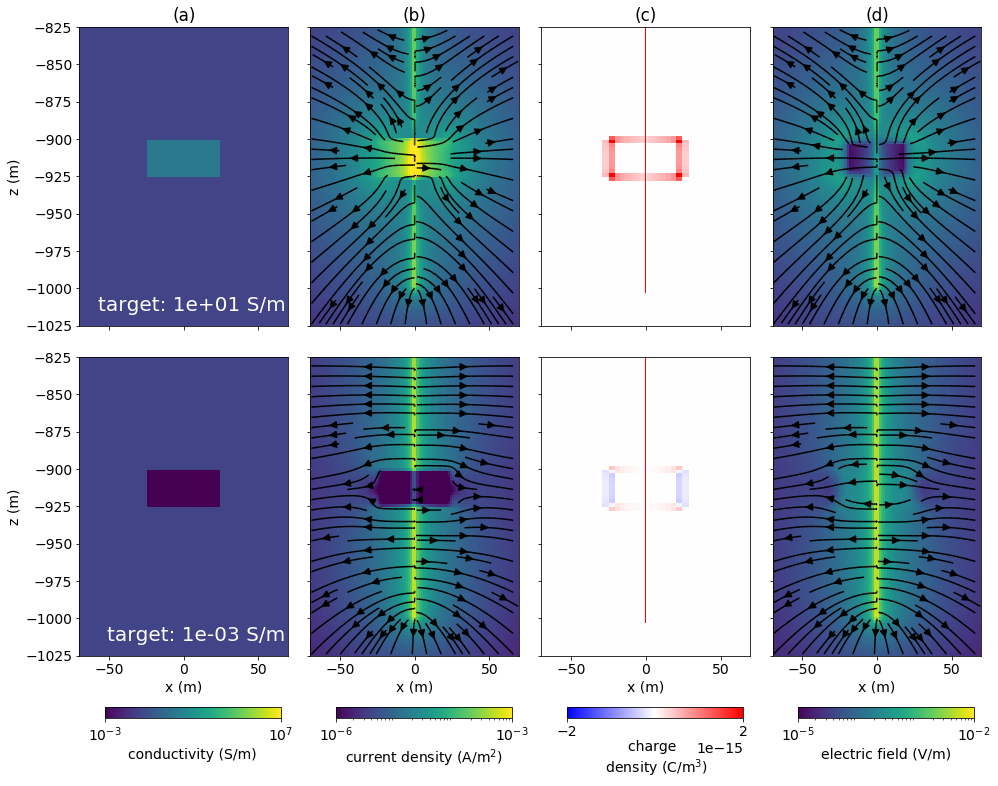
\includegraphics[width=\textwidth]{figures/target_physics.png}
    \end{center}
\caption{
    Cross section showing: (a) electrical conductivity, (b) current density, (c) charge density, and
    (d) electric field for a DC resistivity experiment with a conductive target (top) and a resistive target
    (bottom). The positive electrode is positioned in the casing at the 912.5 m depth.
    The casing is shown by the black line that extends to 1 km
    depth in panel (a).
}
\label{fig:target_physics}
\end{figure}
